\documentclass[12pt,addpoints]{exam}
\usepackage{enumitem}
\usepackage{amsfonts,amssymb,amsmath, amsthm}
\usepackage{graphicx}
\usepackage{systeme}
\usepackage{pgf,tikz,pgfplots}
\pgfplotsset{compat=1.15}
\usepgfplotslibrary{fillbetween}
\usepackage{mathrsfs}
\usetikzlibrary{arrows}
\usetikzlibrary{calc}\author{St John Baptist De La Salle Catholic School, Addis Ababa}
\title{Physics ESSlCE Latex Project}
\usepackage{geometry}
\date{2023}
\geometry{
	a4paper,
	total={170mm,257mm},
	left=15mm,
	right=15mm,
	bottom=20mm,
	top=5mm,
}
\begin{document}
\maketitle
\begin{questions}
	\question The graph below illustrates the position and time for a cat that runs to catch a rat and then returns with it. The cat caught the rat after 2 seconds. What was the cat's average speed as it returned with rat?(2008)
	\begin{center}
		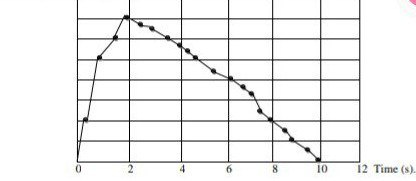
\includegraphics[scale=0.5]{fig1.jpg}
	\end{center}
	\begin{choices}
		\choice Its average return speed was 2m/s.
		\choice Its average return speed was 2m/s.
		\choice Its average return speed was 0.7m/s.
		\choice Its average return speed was 0.9m/s.
	\end{choices}
	\question An airplane flies at speed of 720km/hr at 370 north to west direction. How far does the plane travel to the west in 1 hour?(UEE:2008)\\
	\begin{oneparchoices}
		\choice 432 km.
		\choice 720 km.
		\choice 560 km.
		\choice 504 km.
	\end{oneparchoices}
	\question An airplane travelled from Addis Abeba to Mekele, 780km, in 45 minutes. what was its average speed?(UEE:2008)\\
	\begin{oneparchoices}
		\choice 0.28 m/s.
		\choice 1040 km/hr.
		\choice 17.3 m/min.
		\choice 585 km/hr.
	\end{oneparchoices}
	\question An example of a body moving with constant speed but still accelerating is: 
	\begin{choices}
	\choice A body moving on a straight road.
	\choice A body moving on a straight rail way track.
	\choice A body moving in a circular path .
	\choice A body falling in a viscous fluid.
	\end{choices}
	\question A student moves along the boundary of a square field of side 10m in 40sec. If he started from one of the corners of the square what will be the magnitude of displacement of the student at the end of 2 minutes and 20 second from his intial position?(UEE:2008)\\
		\begin{oneparchoices}
			\choice 10 m.
			\choice 10$\sqrt2$ m.
			\choice 40 m.
			\choice 30 m.
		\end{oneparchoices}
	\question A cricketer throws a ball vertically upwards with initial speed of 20m/s. How long is it in the air before it returns to the cricketer's hands?(UEE:2009)\\
	\begin{oneparchoices}
		\choice 2 s.
		\choice 10 s.
		\choice 1.5 s.
		\choice 4 s.
	\end{oneparchoices}
	\question Two projectiles are fired from ground level at equal speed but different angles. One is fired at angle of 30 degrees and the other at 60 degrees. The projectile to hit the ground first will be the on fired at (neglect air resistance).(UEE:2006) \\
	\begin{oneparchoices}
		\choice 60 degrees.
		\choice 30 degrees.
		\choice Both hit at the same time.
		\choice Cannot be determined from the given information.
	\end{oneparchoices}
	\question A placekicker must kick a football from a point which is at a distance of 36.0m from the goal. When kicked, the ball leaves the ground with a speed of 20.0m/s at an angle of 53\textdegree to the horizontal. If the ball hits the crossbar of the goal at a height h and bounces back what will be the height of the crossbar?(UEE:2006)\\
	\begin{oneparchoices}
		\choice 2.45 m.
		\choice 2.85 m.
		\choice 3.00 m.
		\choice 3.15 m.
	\end{oneparchoices}
	\question A body moving with constant acceleration covers the distance between to point 60m apart in 5s. Its velocity at it passes the second point is 15m/s. What is the acceleration?(UEE:2006)\\
	\begin{oneparchoices}
		\choice $3m/s^2.$
		\choice $2.4m/s^2.$
		\choice $1.8m/s^2.$
		\choice $1.2m/s^2.$
	\end{oneparchoices}
	\question If a long distance athlete leaves the ground at an angle of 37\textdegree above the horizontal surface at a speed of 10m/s, how far does he jump in the horizontal direction?(UEE:2007)\\
	\begin{oneparchoices}
		\choice 4.8 m.
		\choice 6 m.
		\choice 9.6 m.
		\choice 12 m.
	\end{oneparchoices}
	\question A woman is rotating a bucket of water in a vertical circle of radius 0.9m, the mass of bucket and water 5kg. What is the bucket's minimum speed at the top of the circle if no water is if no water is to spill out?(UEE:2007).\\
	\begin{oneparchoices}
		\choice 0.
		\choice 1 m/s.
		\choice 3 m/s.
		\choice 9 m/s.
	\end{oneparchoices}
	\question which one of the following statement is correct?(UEE:2007)
	\begin{choices}
		\choice An object moving towards the east cannot have acceleration towards west.
		\choice If the average velocities of an object zero in some time interval, the average speed of the object for that time interval is also zero.
		\choice The velocity-time graph of an object moving with constant acceleration is parallel to the time axis.
		\choice An object having zero velocity can have acceleration different from zero.
	\end{choices}
	\question An object moving with uniform acceleration has a velocity of 12m/s in the positive x direction when its x coordinate is 3cm. If its x coordinate 2 sec. Later is -5 cm, what is its acceleration?(UEE:2005). 
	\begin{oneparchoices}
		\choice $-12 m/s^2.$
		\choice $-13 m/s^2.$
		\choice $-16 m/s^2.$
		\choice $12 m/s^2.$
	\end{oneparchoices}
	\question What is the direction to which a fish must push the water  with its fins in order to propel eastward?(UEE:2005)\\
	\begin{oneparchoices}
		\choice eastward.
		\choice upward.
		\choice westward.
		\choice downward.
	\end{oneparchoices}
	\question A woman driving a 2000kg car along a level road at 30m/s takes her foot off the gas to see how far her car will roll before it slows to a stop. She discovers that it takes 150m. What is the greatest force of friction acting on the car?(UEE:2005).\\
	\begin{oneparchoices}
		\choice 9000N.
		\choice 6000N.
		\choice 3000N.
		\choice 400N.
	\end{oneparchoices}
	\question The coordinate of a particle in meters is given by $ x(t)=25t-3t^2$, where the time t is in seconds. At what value t will the particle become momentarily at rest?(UEE:2005)
	\begin{oneparchoices}\\
		\choice 2.87 s.
		\choice 1.67 s.
		\choice 0.6 s.
		\choice 0.36 s.
	\end{oneparchoices}
	\question A force \textbf{F} of magnitude 20N is applied to a block of mass 2 kg that lies on a rough, horizontal surface as shown in figure below. The coefficient of kinetic friction between the block and surface is 0.4.What is the magnitude of the acceleration of the block?(UEE:2007) 
	\begin{center}
		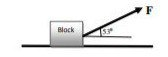
\includegraphics[scale=0.6]{fig2.jpq.jpg}
	\end{center}
	\begin{oneparchoices}
	\choice $10m/s^2.$
	\choice $5.2m/s^2.$
	\choice $4m/s^2.$
	\choice $2.8m/s^2.$
	\end{oneparchoices}
\end{questions}
\end{document}




